\documentclass[tikz]{standalone}
\usepackage{tikz}
\usetikzlibrary{plotmarks}
\usetikzlibrary{math}

\usepackage{pgfplots}
\pgfplotsset{compat=newest}

\newcommand*{\gridlimit}{4.99}

\begin{document}
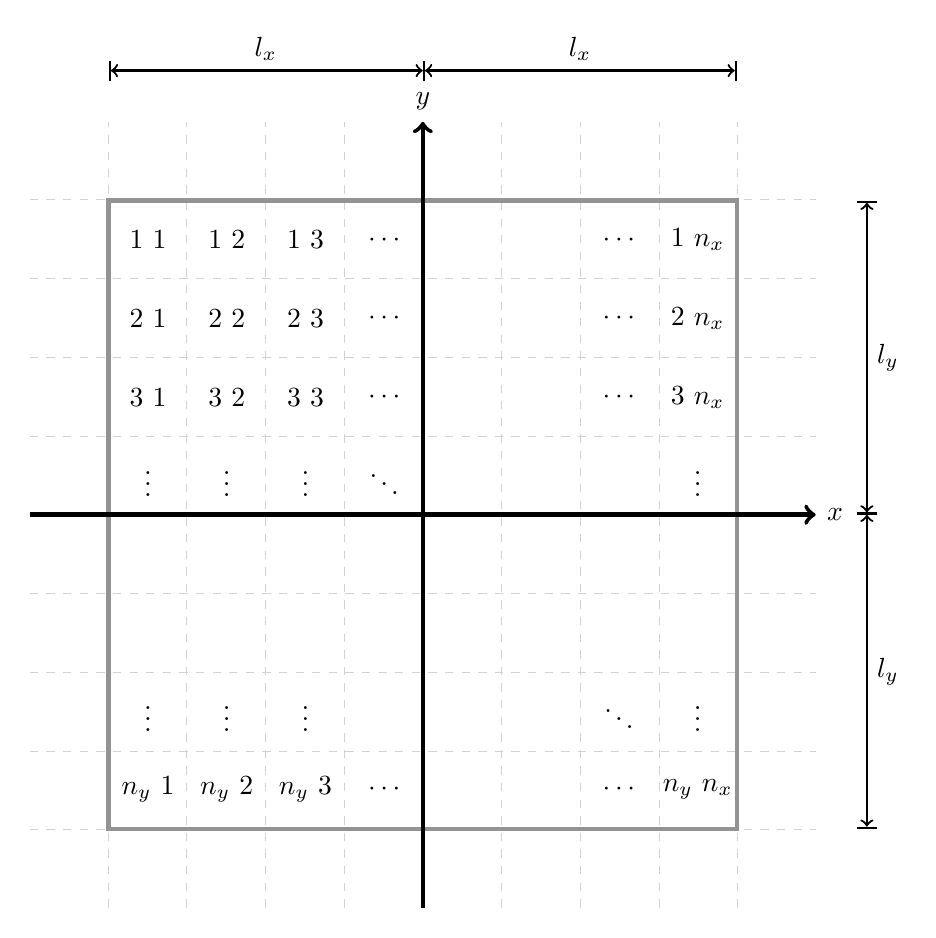
\begin{tikzpicture}
    % grid lines
    \draw[help lines, color=gray!35, dashed, step=1] (-\gridlimit, -\gridlimit) grid (\gridlimit, \gridlimit);
    % square space limit
    \draw[ultra thick, color=gray!85] (-\gridlimit+1, -\gridlimit+1) -- (\gridlimit-1, -\gridlimit+1) -- (\gridlimit-1, \gridlimit-1) -- (-\gridlimit+1, \gridlimit-1) -- cycle;
    % first row
    \node at (-\gridlimit+1.5,\gridlimit-1.5) {$1\ 1$};
    \node at (-\gridlimit+2.5,\gridlimit-1.5) {$1\ 2$};
    \node at (-\gridlimit+3.5,\gridlimit-1.5) {$1\ 3$};
    \node at (-\gridlimit+4.5,\gridlimit-1.5) {$\cdots$};
    \node at (\gridlimit-2.5,\gridlimit-1.5) {$\cdots$};
    \node at (\gridlimit-1.5,\gridlimit-1.5) {$1\ n_x$};
    % second row
    \node at (-\gridlimit+1.5,\gridlimit-2.5) {$2\ 1$};
    \node at (-\gridlimit+2.5,\gridlimit-2.5) {$2\ 2$};
    \node at (-\gridlimit+3.5,\gridlimit-2.5) {$2\ 3$};
    \node at (-\gridlimit+4.5,\gridlimit-2.5) {$\cdots$};
    \node at (\gridlimit-2.5,\gridlimit-2.5) {$\cdots$};
    \node at (\gridlimit-1.5,\gridlimit-2.5) {$2\ n_x$};
    % third row
    \node at (-\gridlimit+1.5,\gridlimit-3.5) {$3\ 1$};
    \node at (-\gridlimit+2.5,\gridlimit-3.5) {$3\ 2$};
    \node at (-\gridlimit+3.5,\gridlimit-3.5) {$3\ 3$};
    \node at (-\gridlimit+4.5,\gridlimit-3.5) {$\cdots$};
    \node at (\gridlimit-2.5,\gridlimit-3.5) {$\cdots$};
    \node at (\gridlimit-1.5,\gridlimit-3.5) {$3\ n_x$};
    % fourth row
    \node at (-\gridlimit+1.5,\gridlimit-4.5) {$\vdots$};
    \node at (-\gridlimit+2.5,\gridlimit-4.5) {$\vdots$};
    \node at (-\gridlimit+3.5,\gridlimit-4.5) {$\vdots$};
    \node at (-\gridlimit+4.5,\gridlimit-4.5) {$\ddots$};
    \node at (\gridlimit-1.5,\gridlimit-4.5) {$\vdots$};
    % one before last row
    \node at (-\gridlimit+1.5,-\gridlimit+2.5) {$\vdots$};
    \node at (-\gridlimit+2.5,-\gridlimit+2.5) {$\vdots$};
    \node at (-\gridlimit+3.5,-\gridlimit+2.5) {$\vdots$};
    \node at (\gridlimit-2.5,-\gridlimit+2.5) {$\ddots$};
    \node at (\gridlimit-1.5,-\gridlimit+2.5) {$\vdots$};
    % last row
    \node at (-\gridlimit+1.5,-\gridlimit+1.5) {$n_y\ 1$};
    \node at (-\gridlimit+2.5,-\gridlimit+1.5) {$n_y\ 2$};
    \node at (-\gridlimit+3.5,-\gridlimit+1.5) {$n_y\ 3$};
    \node at (-\gridlimit+4.5,-\gridlimit+1.5) {$\cdots$};
    \node at (\gridlimit-2.5,-\gridlimit+1.5) {$\cdots$};
    \node at (\gridlimit-1.5,-\gridlimit+1.5) {$n_y\ n_x$};
    % x axis
    \draw[->, ultra thick] (-\gridlimit, 0) -- (\gridlimit, 0) node[right] {$x$};
    % y axis
    \draw[->, ultra thick] (0, -\gridlimit) -- (0, \gridlimit) node[above] {$y$};
    % ly lengths
    \draw[|<->|, thick] (\gridlimit+0.65, 0) -- node[right] {$l_y$} (\gridlimit+0.65, \gridlimit-1);
    \draw[<->|, thick] (\gridlimit+0.65, 0) -- node[right] {$l_y$} (\gridlimit+0.65, -\gridlimit+1);
    %lx lengths
    \draw[|<->|, thick] (0, \gridlimit+0.65) -- node[above] {$l_x$} (\gridlimit-1, \gridlimit+0.65);
    \draw[<->|, thick] (0, \gridlimit+0.65) -- node[above] {$l_x$} (-\gridlimit+1, \gridlimit+0.65);
\end{tikzpicture}
\end{document}
